\documentclass[border=5pt]{standalone}
\usepackage{tikz}
\usepackage{pgfplots}
\pgfplotsset{compat=1.18}
\usepackage{amsmath}
\usepackage{amssymb}
\usepackage{xcolor}

% Brand colors
\definecolor{tiger}{HTML}{FF5A00}
\definecolor{fire}{HTML}{FF4D00}
\definecolor{flicker}{HTML}{DC4B07}
\definecolor{steel}{HTML}{878F92}
\definecolor{gunmetal}{HTML}{122128}
\definecolor{panelc}{HTML}{202E35}

% Figure colors
\definecolor{darknavy}{HTML}{122128}
\definecolor{forgisorange}{HTML}{FF5A00}
\definecolor{forgisfire}{HTML}{FF4D00}
\definecolor{forgisflicker}{HTML}{DC4B07}
\definecolor{figblue}{HTML}{3A7BD5}
\definecolor{figgreen}{HTML}{2ECC71}
\definecolor{figsteel}{HTML}{878F92}
\definecolor{panelbg}{HTML}{F0F4F8}
\definecolor{warmamber}{HTML}{FFF3CD}

% Level colors
\definecolor{L1bg}{HTML}{E0F2F1}
\definecolor{L1border}{HTML}{00796B}
\definecolor{L2bg}{HTML}{FFF8E1}
\definecolor{L2border}{HTML}{F57F17}
\definecolor{L3bg}{HTML}{F3E5F5}
\definecolor{L3border}{HTML}{6A1B9A}
\definecolor{L4bg}{HTML}{FFEBEE}
\definecolor{L4border}{HTML}{B71C1C}

% Panel tint colors from description
\definecolor{L1tint}{HTML}{FB9E6C}
\definecolor{L2tint}{HTML}{FF7F3A}
\definecolor{L3tint}{HTML}{FF5A00}

\usetikzlibrary{calc,decorations.pathreplacing,arrows.meta,patterns,positioning,shapes.geometric,backgrounds,fit}

\begin{document}
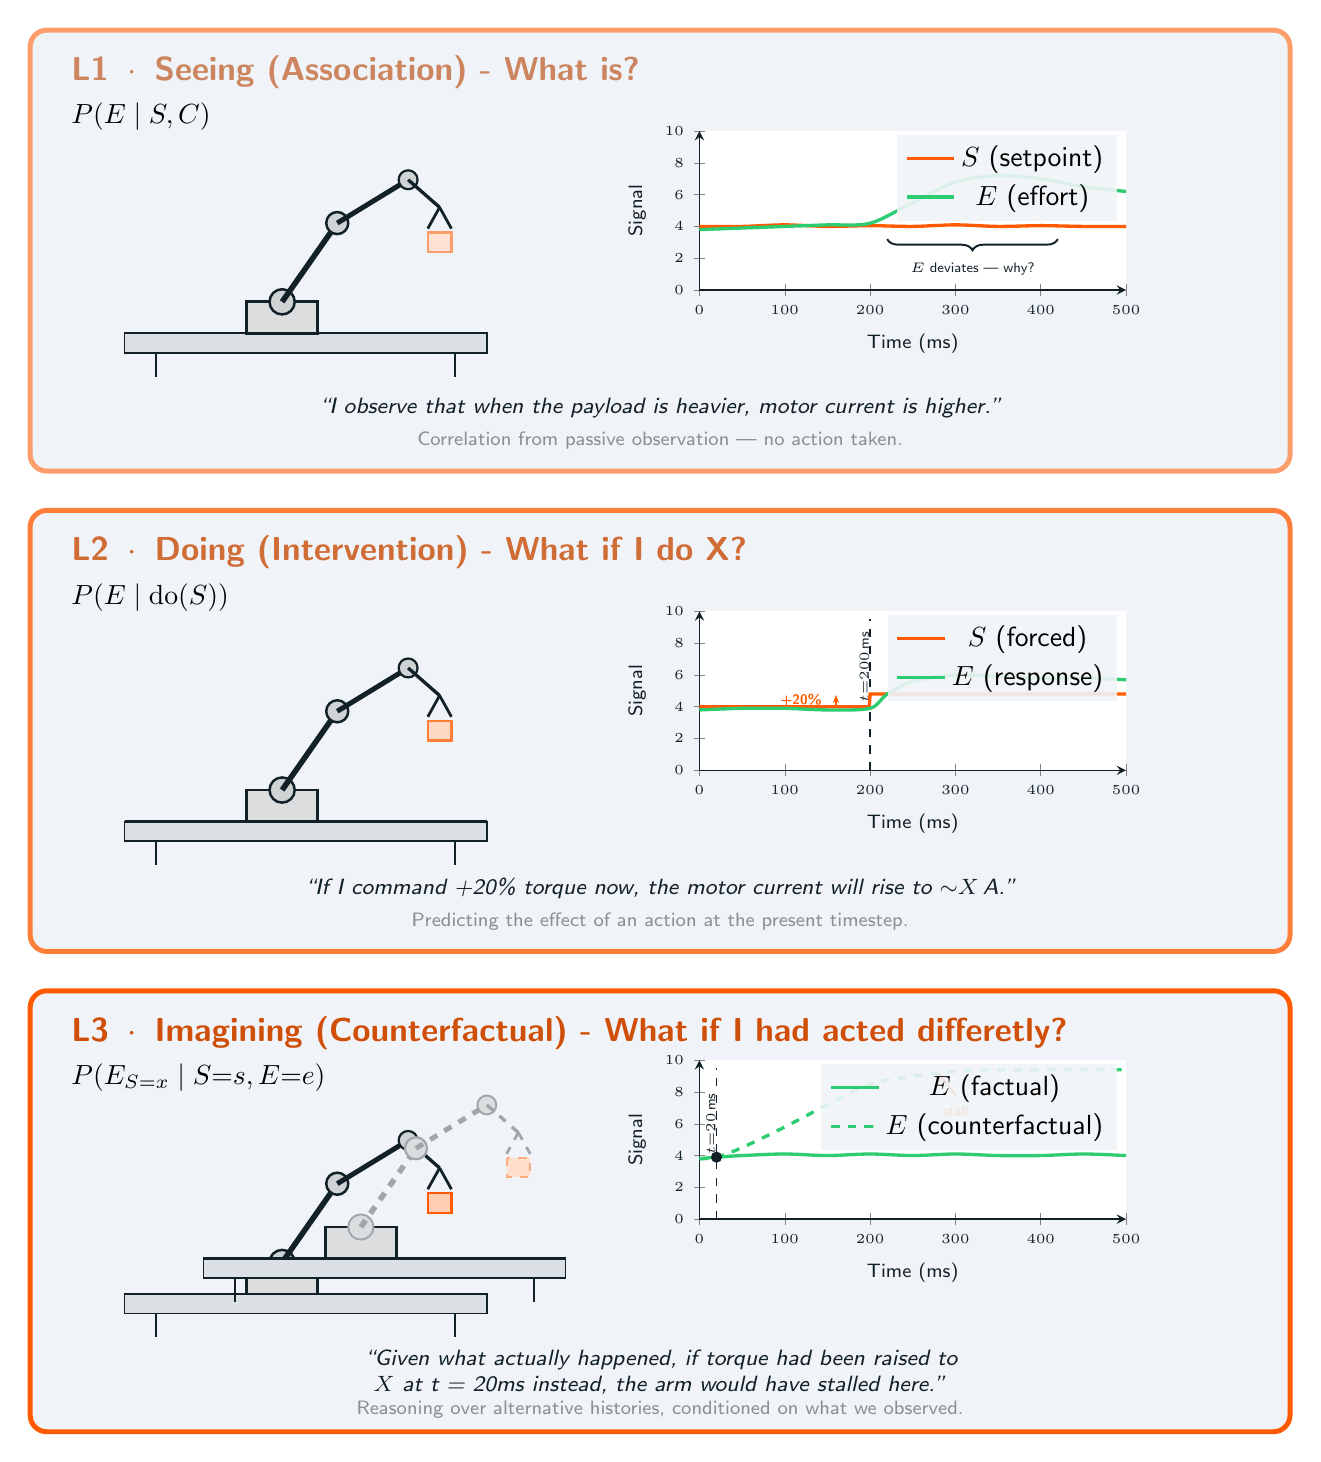
\begin{tikzpicture}[
  every node/.style={font=\sffamily},
]

\def\panelw{16.0}
\def\panelh{5.6}
\def\panelgap{0.5}

% Coordinates for panel centers
\coordinate (P1center) at (0, 0);
\coordinate (P2center) at (0, -\panelh-\panelgap);
\coordinate (P3center) at (0, -2*\panelh-2*\panelgap);


% ============================================================
% MACRO: Draw robot arm
% ============================================================
\newcommand{\drawrobot}[4]{
  % #1=x, #2=y, #3=style(0=normal,1=intervention,2=ghost), #4=accent
  \begin{scope}[shift={(#1,#2)}]
    % Workbench
    \fill[panelbg!80!figsteel] (-2.0,-1.6) rectangle (2.6,-1.35);
    \draw[darknavy, line width=0.8pt] (-2.0,-1.35) -- (2.6,-1.35);
    \draw[darknavy, line width=0.6pt] (-2.0,-1.6) rectangle (2.6,-1.35);
    % Bench legs
    \draw[darknavy, line width=0.7pt] (-1.6,-1.6) -- (-1.6,-1.9);
    \draw[darknavy, line width=0.7pt] (2.2,-1.6) -- (2.2,-1.9);
    
    % Robot base
    \fill[figsteel!30] (-0.45,-1.35) rectangle (0.45,-0.95);
    \draw[darknavy, line width=1pt] (-0.45,-1.35) rectangle (0.45,-0.95);
    
    % Joint 1 (base rotation)
    \ifnum#3=2
      \filldraw[darknavy!15, draw=darknavy!40, line width=0.7pt] (0,-0.95) circle (0.16);
    \else
      \filldraw[darknavy!20, draw=darknavy, line width=0.9pt] (0,-0.95) circle (0.16);
    \fi
    
    % Link 1
    \ifnum#3=2
      \draw[darknavy!40, line width=2pt, dashed] (0,-0.95) -- (0.7,0.05);
    \else
      \draw[darknavy, line width=2pt] (0,-0.95) -- (0.7,0.05);
    \fi
    
    % Joint 2
    \ifnum#3=2
      \filldraw[darknavy!15, draw=darknavy!40, line width=0.8pt] (0.7,0.05) circle (0.14);
    \else
      \filldraw[darknavy!20, draw=darknavy, line width=0.9pt] (0.7,0.05) circle (0.14);
    \fi
    
    % Link 2
    \ifnum#3=2
      \draw[darknavy!40, line width=1.8pt, dashed] (0.7,0.05) -- (1.6,0.6);
    \else
      \draw[darknavy, line width=1.8pt] (0.7,0.05) -- (1.6,0.6);
    \fi
    
    % Joint 3 (wrist)
    \ifnum#3=2
      \filldraw[darknavy!15, draw=darknavy!40, line width=0.7pt] (1.6,0.6) circle (0.12);
    \else
      \filldraw[darknavy!20, draw=darknavy, line width=0.8pt] (1.6,0.6) circle (0.12);
    \fi
    
    % End effector / gripper
    \ifnum#3=2
      \draw[darknavy!40, line width=1.2pt, dashed] (1.6,0.6) -- (2.0,0.25);
      \draw[darknavy!40, line width=1pt, dashed] (2.0,0.25) -- (1.85,-0.02);
      \draw[darknavy!40, line width=1pt, dashed] (2.0,0.25) -- (2.15,-0.02);
    \else
      \draw[darknavy, line width=1.2pt] (1.6,0.6) -- (2.0,0.25);
      \draw[darknavy, line width=1pt] (2.0,0.25) -- (1.85,-0.02);
      \draw[darknavy, line width=1pt] (2.0,0.25) -- (2.15,-0.02);
    \fi
    
    % Payload (box)
    \ifnum#3=2
      \fill[#4!20] (1.85,-0.07) rectangle (2.15,-0.32);
      \draw[#4!50, line width=0.7pt, dashed] (1.85,-0.07) rectangle (2.15,-0.32);
    \else
      \fill[#4!30] (1.85,-0.07) rectangle (2.15,-0.32);
      \draw[#4, line width=0.8pt] (1.85,-0.07) rectangle (2.15,-0.32);
    \fi
  \end{scope}
}

% ============================================================
% PANEL 1: L1 · Seeing (Association)
% ============================================================
\begin{scope}[shift={(P1center)}]
  % Panel background
  \fill[panelbg, rounded corners=6pt] (-\panelw/2, -\panelh/2) rectangle (\panelw/2, \panelh/2);
  \draw[L1tint, line width=1.8pt, rounded corners=6pt] (-\panelw/2, -\panelh/2) rectangle (\panelw/2, \panelh/2);
  
  \node[anchor=north west, font=\sffamily\bfseries\large, L1tint!80!darknavy] at (-\panelw/2+0.4, \panelh/2-0.2) {L1 \,$\cdot$\, Seeing (Association) - What is?};
  \node[anchor=north west, font=\sffamily, text=black] at (-\panelw/2+0.4, \panelh/2-0.8) {$P(E \mid S, C)$};
    
  % Robot arm (normal)
  \drawrobot{-4.8}{0.3}{0}{L1tint}
  
  % Plot area (Centered)
  \begin{scope}[shift={(0.5, -0.5)}]
    \begin{axis}[
      width=7.0cm, height=3.6cm,
      xmin=0, xmax=500, ymin=0, ymax=10,
      xlabel={Time (ms)}, ylabel={Signal},
      xlabel style={font=\sffamily\scriptsize, darknavy},
      ylabel style={font=\sffamily\scriptsize, darknavy},
      tick label style={font=\sffamily\tiny, darknavy},
      xtick={0,100,200,300,400,500},
      ytick={0,2,4,6,8,10},
      axis lines=left,
      axis line style={darknavy, line width=0.5pt},
      legend style={at={(0.98,0.98)}, anchor=north east, font=\sffamily\tiny,
        draw=none, fill=panelbg, fill opacity=0.9, text opacity=1,
        row sep=1pt, legend columns=1},
      clip=true,
      axis background/.style={fill=white},
    ]
      % Setpoint S (orange)
      \addplot[forgisorange, line width=1.2pt, smooth] coordinates {
        (0,4) (50,4) (100,4.1) (150,4) (200,4.05) (250,4) (300,4.1) (350,4) (400,4.05) (450,4) (500,4)
      };
      \addlegendentry{$S$ (setpoint)}
      
      % Effort E (green) with deviation
      \addplot[figgreen, line width=1.2pt, smooth] coordinates {
        (0,3.8) (50,3.9) (100,4.0) (150,4.1) (200,4.2) (250,5.5) (300,6.8) (350,7.2) (400,7.0) (450,6.5) (500,6.2)
      };
      \addlegendentry{$E$ (effort)}
      
      % Question bracket on deviation segment
      \draw[decorate, decoration={brace, amplitude=4pt, mirror}, darknavy, line width=0.7pt]
        (axis cs:220,3.2) -- (axis cs:420,3.2)
        node[midway, below=5pt, font=\sffamily\tiny, darknavy] {$E$ deviates --- why?};
    \end{axis}
  \end{scope}
  
  % Tag line
  \node[anchor=south, font=\sffamily\footnotesize\itshape, darknavy, text width=14.5cm, align=center]
    at (0, -\panelh/2+0.55) {``I observe that when the payload is heavier, motor current is higher.''};
  % Subtitle
  \node[anchor=south, font=\sffamily\scriptsize, figsteel, text width=14.5cm, align=center]
    at (0, -\panelh/2+0.15) {Correlation from passive observation --- no action taken.};
\end{scope}

% ============================================================
% PANEL 2: L2 · Doing (Intervention)
% ============================================================
\begin{scope}[shift={(P2center)}]
  % Panel background
  \fill[panelbg, rounded corners=6pt] (-\panelw/2, -\panelh/2) rectangle (\panelw/2, \panelh/2);
  \draw[L2tint, line width=1.8pt, rounded corners=6pt] (-\panelw/2, -\panelh/2) rectangle (\panelw/2, \panelh/2);
  
  % Título y texto de saludo
  \node[anchor=north west, font=\sffamily\bfseries\large, L2tint!80!darknavy] at (-\panelw/2+0.4, \panelh/2-0.2) {L2 \,$\cdot$\, Doing (Intervention) - What if I do X?};
  \node[anchor=north west, font=\sffamily, text=black] at (-\panelw/2+0.4, \panelh/2-0.8) {$P(E \mid \mathrm{do}(S))$};
    
  % Robot arm (normal with intervention arrow)
  \drawrobot{-4.8}{0.2}{0}{L2tint}
    
  % Plot area (Centered)
  \begin{scope}[shift={(0.5, -0.5)}]
    \begin{axis}[
      width=7.0cm, height=3.6cm,
      xmin=0, xmax=500, ymin=0, ymax=10,
      xlabel={Time (ms)}, ylabel={Signal},
      xlabel style={font=\sffamily\scriptsize, darknavy},
      ylabel style={font=\sffamily\scriptsize, darknavy},
      tick label style={font=\sffamily\tiny, darknavy},
      xtick={0,100,200,300,400,500},
      ytick={0,2,4,6,8,10},
      axis lines=left,
      axis line style={darknavy, line width=0.5pt},
      legend style={at={(0.98,0.98)}, anchor=north east, font=\sffamily\tiny,
        draw=none, fill=panelbg, fill opacity=0.9, text opacity=1,
        row sep=1pt, legend columns=1},
      clip=true,
      axis background/.style={fill=white},
    ]
      % Intervention line
      \draw[darknavy, line width=0.7pt, dashed] (axis cs:200,0) -- (axis cs:200,9.5);
      \node[font=\sffamily\tiny, darknavy, anchor=south, rotate=90] at (axis cs:210,6.5) {$t{=}200$\,ms};
      
      % Setpoint S (orange), forcibly altered at t=200
      \addplot[forgisorange, line width=1.2pt] coordinates {
        (0,4) (50,4) (100,4) (150,4) (199,4) (200,4.8) (250,4.8) (300,4.8) (350,4.8) (400,4.8) (450,4.8) (500,4.8)
      };
      \addlegendentry{$S$ (forced)}
      
      % Effort E (green) responding
      \addplot[figgreen, line width=1.2pt, smooth] coordinates {
        (0,3.8) (50,3.9) (100,3.9) (150,3.8) (200,3.9) (220,4.8) (250,5.6) (300,6.0) (350,5.9) (400,5.8) (450,5.8) (500,5.7)
      };
      \addlegendentry{$E$ (response)}
      
      % Annotation for +20%
      \draw[-{Stealth[length=3pt]}, forgisorange, line width=0.9pt]
        (axis cs:160,4.05) -- (axis cs:160,4.75);
      \node[font=\sffamily\tiny\bfseries, forgisorange, anchor=east] at (axis cs:155,4.4) {+20\%};
    \end{axis}
  \end{scope}
  
  % Tag line
  \node[anchor=south, font=\sffamily\footnotesize\itshape, darknavy, text width=14.5cm, align=center]
    at (0, -\panelh/2+0.55) {``If I command +20\% torque now, the motor current will rise to ${\sim}X$\,A.''};
  % Subtitle
  \node[anchor=south, font=\sffamily\scriptsize, figsteel, text width=14.5cm, align=center]
    at (0, -\panelh/2+0.15) {Predicting the effect of an action at the present timestep.};
\end{scope}

% ============================================================
% PANEL 3: L3 · Imagining (Counterfactual)
% ============================================================
\begin{scope}[shift={(P3center)}]
  % Panel background
  \fill[panelbg, rounded corners=6pt] (-\panelw/2, -\panelh/2) rectangle (\panelw/2, \panelh/2);
  \draw[L3tint, line width=1.8pt, rounded corners=6pt] (-\panelw/2, -\panelh/2) rectangle (\panelw/2, \panelh/2);
  
  \node[anchor=north west, font=\sffamily\bfseries\large, L3tint!80!darknavy] at (-\panelw/2+0.4, \panelh/2-0.2) {L3 \,$\cdot$\, Imagining (Counterfactual) - What if I had acted differetly?};
  \node[anchor=north west, font=\sffamily, text=black] at (-\panelw/2+0.4, \panelh/2-0.8) {$P(E_{S=x} \mid S{=}s, E{=}e)$};

  % Real robot arm (solid)
  \drawrobot{-4.8}{0.3}{0}{L3tint}
  
  % Ghost robot arm (dashed, shifted)
  \drawrobot{-3.8}{0.75}{2}{L3tint}
  
  % Plot area (Centered)
  \begin{scope}[shift={(0.5, -0.1)}]
    \begin{axis}[
      width=7.0cm, height=3.6cm,
      xmin=0, xmax=500, ymin=0, ymax=10,
      xlabel={Time (ms)}, ylabel={Signal},
      xlabel style={font=\sffamily\scriptsize, darknavy},
      ylabel style={font=\sffamily\scriptsize, darknavy},
      tick label style={font=\sffamily\tiny, darknavy},
      xtick={0,100,200,300,400,500},
      ytick={0,2,4,6,8,10},
      axis lines=left,
      axis line style={darknavy, line width=0.5pt},
      legend style={at={(0.98,0.98)}, anchor=north east, font=\sffamily\tiny,
        draw=none, fill=panelbg, fill opacity=0.9, text opacity=1,
        row sep=1pt, legend columns=1},
      clip=true,
      axis background/.style={fill=white},
    ]
      % Intervention line at t=20
      \draw[darknavy, line width=0.7pt, dashed] (axis cs:20,0) -- (axis cs:20,9.5);
      \node[font=\sffamily\tiny, darknavy, anchor=south, rotate=90] at (axis cs:30,6) {$t{=}20$\,ms};
      
      % Factual E (solid green)
      \addplot[figgreen, line width=1.2pt, smooth] coordinates {
        (0,3.8) (20,3.9) (50,4.0) (100,4.1) (150,4.0) (200,4.1) (250,4.0) (300,4.1) (350,4.0) (400,4.0) (450,4.1) (500,4.0)
      };
      \addlegendentry{$E$ (factual)}
      
      % Counterfactual E (dashed green)
      \addplot[figgreen, line width=1.2pt, dashed, smooth] coordinates {
        (0,3.8) (20,3.9) (50,4.5) (100,5.8) (150,7.2) (200,8.5) (250,9.0) (300,9.3) (350,9.4) (400,9.4) (450,9.4) (500,9.4)
      };
      \addlegendentry{$E$ (counterfactual)}
      
      % Stall annotation
      \draw[-{Stealth[length=3pt]}, L3tint, line width=0.8pt]
        (axis cs:300,7.8) -- (axis cs:280,9.2);
      \node[font=\sffamily\tiny\bfseries, L3tint, anchor=north] at (axis cs:300,7.7) {stall};
      
      % Branch point
      \filldraw[darknavy] (axis cs:20,3.9) circle (1.8pt);
    \end{axis}
  \end{scope}
  
  % Tag line
  \node[anchor=south, font=\sffamily\footnotesize\itshape, darknavy, text width=14.5cm, align=center]
    at (0, -\panelh/2+0.35) {``Given what actually happened, if torque had been raised to $X$ at t = 20ms instead, the arm would have stalled here.''};
  % Subtitle
  \node[anchor=south, font=\sffamily\scriptsize, figsteel, text width=14.5cm, align=center]
    at (0, -\panelh/2+0.05) {Reasoning over alternative histories, conditioned on what we observed.};
\end{scope}

\end{tikzpicture}
\end{document}